\chapter*{Metodología Experimental} %15 por ciento
\addcontentsline{toc}{chapter}{Metodología Experimental}
La investigación se llevará a cabo mediante un diseño de revisión bibliográfica, complementado con simulaciones que permitan entender y analizar el funcionamiento de los amplificadores de bloqueo en la amplificación de señales débiles. Este enfoque permitirá reunir información teórica y práctica sobre el tema, facilitando un análisis más profundo. La selección de fuentes incluirá una variedad de materiales relevantes, tales como libros especializados, artículos científicos revisados por pares, patentes y bases de datos académicas. Estas fuentes se elegirán por su calidad, relevancia y actualidad, asegurando que la información recopilada sea sólida y pertinente para el estudio.\\
\\
La recolección de datos se realizará a partir de la información obtenida de las simulaciones. Estas simulaciones se diseñarán para replicar diferentes escenarios en los que se utilizan amplificadores de bloqueo, permitiendo observar su comportamiento bajo diversas condiciones y ajustando los parámetros necesarios para maximizar la amplificación de señales débiles.\\
\\
Finalmente, se llevará a cabo un análisis de datos utilizando técnicas estadísticas y cualitativas. Se emplearán métodos estadísticos para evaluar la efectividad de las configuraciones de los amplificadores de bloqueo, así como análisis cualitativos para interpretar los resultados de las simulaciones y la información obtenida de la revisión bibliográfica. Este enfoque integrador permitirá extraer conclusiones significativas sobre el funcionamiento y la optimización de los amplificadores de bloqueo en la detección de señales débiles.
%%%%%%%%%%%%%%%%%%%%%%%%%%%%%%%%%%%%%%%%%%%%%%%%%%%%%%%%%%%%%%%%
\section*{Desarrollo del problema}
\addcontentsline{toc}{section}{Desarrollo del problema} %Eduardo

El problema central de este proyecto es la necesidad de amplificar señales extremadamente débiles, que suelen estar sumergidas en ruido de fondo, un reto común en la detección de radiación y en otras áreas de la física experimental. La amplificación de estas señales es crucial para obtener mediciones precisas y confiables, pero lograrlo presenta desafíos significativos. Los amplificadores de bloqueo han sido una solución eficaz para extraer señales débiles en condiciones ruidosas, sin embargo, su correcta configuración y operación es compleja. La dependencia de la frecuencia de referencia y la sensibilidad al ruido limitan su efectividad en situaciones donde las señales fluctúan o son dinámicas, lo que plantea la necesidad de una optimización cuidadosa de sus parámetros operativos.\\
\\
Se plantea como hipótesis que una configuración optimizada del amplificador de bloqueo, ajustando adecuadamente los parámetros de frecuencia y sensibilidad al ruido, permitirá una amplificación eficiente de señales débiles, minimizando las limitaciones técnicas asociadas. Además, se espera que la mejora en la configuración maximice el rendimiento del amplificador en la detección de señales débiles en presencia de ruido.\\
\\
Para resolver este problema, es necesario responder varias preguntas: ¿Qué configuraciones y ajustes permiten una amplificación óptima de señales débiles utilizando un amplificador de bloqueo?, ¿Cuáles son los principales factores que limitan el rendimiento de estos dispositivos en la detección de señales?, ¿Qué tipos de señales se benefician más del uso de amplificadores de bloqueo y cómo se pueden adaptar los parámetros para trabajar eficazmente con diferentes niveles de ruido de fondo?.




\subsection*{Desarrollo experimental}
\addcontentsline{toc}{subsection}{Desarrollo experimental}

Dado que esta investigación se basa en una revisión bibliográfica, se utilizará el simulador LIA Simulation para ayudar a interpretar el funcionamiento de los amplificadores de bloqueo y proporcionar una comprensión más profunda de su operación en la amplificación de señales débiles. Este enfoque permitirá abordar las hipótesis planteadas y responder las preguntas de investigación de manera efectiva, para lo cual se realizaran 3 etapas; una prueba previa en el cual se familiarizara la interfaz y configuración del simulador, una serie de simulaciones en las cuales se estudiara los efectos del amplificador y como ultima etapa una posprueba para poner a prueba los conocimientos aprendidos en las 2 etapas anteriores. 

\subsubsection{Prueba Previa}
Para el análisis del simulador, es necesario conocer los siguientes símbolos, mostrados en la Tabla \ref{tab:3}.

\begin{table}[h]
\centering
\resizebox{\columnwidth}{!}{%
\begin{tabular}{cccc}
\toprule
Símbolos & Significado  \\
\midrule
$f_S$ & Frecuencia de la señal de entrada\\
$f_R$ & Frecuencia de la referencia de bloqueo \\
$f_C$ & Frecuencia de la señal de entrada sinusoidal adicional (o ruido coherente) \\
$f_{AM}$ & Frecuencia de la modulación de amplitud de la señal de entrada\\
$A_S$ & Amplitud de la señal de entrada\\
$A_C$ & Amplitud de la señal de entrada sinusoidal adicional (o ruido coherente)\\
$P_{AM}$ & Porcentaje de amplitud agregado a la amplitud como modulación de amplitud\\
$\eta$ & Definido aquí (Aumentar este valor aumenta la intensidad de este ruido)\\
$\phi$ & Ángulo de fase de la señal de entrada con respecto a la señal de referencia\\
$\tau$ & Constante de tiempo (el “ms” que aparece en esta simulación significa milisegundos) \\
$V_{MX}$ & Salida del amplificador lock-in en fase con la referencia antes del filtro de paso bajo\\
$V_{MY}$ & Salida del amplificador lock-in desfasada con la referencia antes del filtro de paso bajo\\
$V_{OutX}$ & Salida del amplificador lock-in en fase con la referencia\\
$V_{OutY}$ & Salida del amplificador lock-in desfasada con respecto a la referencia\\
\bottomrule
\end{tabular}%
}
\caption{Variables utilizadas en el simulador}
\label{tab:3}
\end{table}

Ahora podemos realizar las siguientes demostraciones del simulador.

\begin{table}[H]
\centering
\resizebox{0.55\columnwidth}{!}{ % Ajusta el tamaño al 90% del ancho de la columna
\begin{tabular}{c|c|c} % Definir columnas
    \hline
    \textbf{Variable} & \textbf{Valor} & \textbf{Resultados} \\
    \hline
    $f_s$   & 80 & \multirow{6}{*}{%
    \begin{minipage}{.25\textwidth}
    \centering
    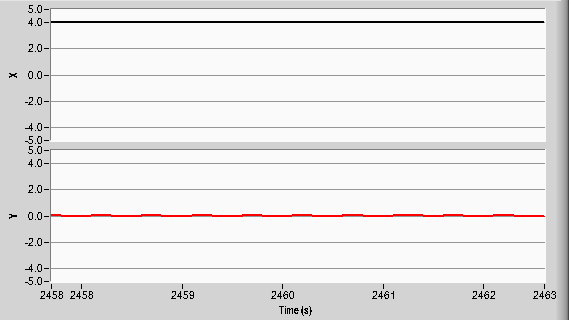
\includegraphics[width=1.2\textwidth]{Chapters/4_Metodología/Imagenes/1.png} \\
    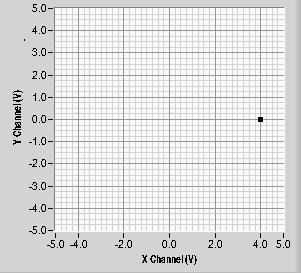
\includegraphics[width=1.2\textwidth]{Chapters/4_Metodología/Imagenes/2.png}
    \end{minipage}} \\
    $f_R$ & 80 \\
    $f_C$ & 60 \\
    $f_{AM}$ & 0\\
    $A_S$ & 4\\
    $A_C$ & 1\\
    $P_{AM}$ & 0\\
    $\eta$ & 0\\
    $\phi$ & 0\\
    $\tau$ & 1 \\
    $V_{MX}$ & 4\\
    $V_{MY}$ & 1\\
    $V_{OutX}$ & 4\\
    $V_{OutY}$ & 0\\
    Entrada sinusoidal & desactivada\\
    Filtro de paso bajo & activado \\
    \hline
\end{tabular}
}
\caption{Variables utilizadas en el simulador con sus respectivas salidas.}
\end{table}

\begin{table}[H]
\centering
\resizebox{0.55\columnwidth}{!}{ % Ajusta el tamaño al 90% del ancho de la columna
\begin{tabular}{c|c|c} % Definir columnas
    \hline
    \textbf{Variable} & \textbf{Valor} & \textbf{Resultados} \\
    \hline
    $f_s$   & 100 & \multirow{6}{*}{%
    \begin{minipage}{.25\textwidth}
    \centering
    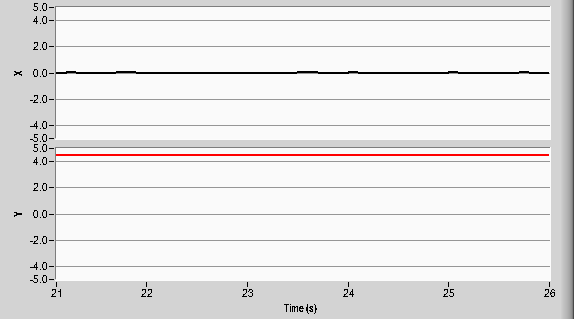
\includegraphics[width=1.2\textwidth]{Chapters/4_Metodología/Imagenes/3.png} \\
    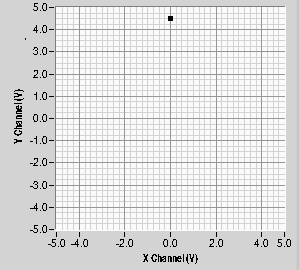
\includegraphics[width=1.2\textwidth]{Chapters/4_Metodología/Imagenes/4.png}
    \end{minipage}} \\
    $f_R$ & 100 \\
    $f_C$ & 60 \\
    $f_{AM}$ & 0\\
    $A_S$ & 4.5\\
    $A_C$ & 1\\
    $P_{AM}$ & 0\\
    $\eta$ & 0\\
    $\phi$ & 90\\
    $\tau$ & 1 \\
    $V_{MX}$ & 4.5\\
    $V_{MY}$ & 1\\
    $V_{OutX}$ & 0\\
    $V_{OutY}$ & 4.5\\
    Entrada sinusoidal & desactivada\\
    Filtro de paso bajo & activado \\
    \hline
\end{tabular}
}
\caption{Variables utilizadas en el simulador con sus respectivas salidas.}
\end{table}

\begin{table}[H]
\centering
\resizebox{0.55\columnwidth}{!}{ % Ajusta el tamaño al 90% del ancho de la columna
\begin{tabular}{c|c|c} % Definir columnas
    \hline
    \textbf{Variable} & \textbf{Valor} & \textbf{Resultados} \\
    \hline
    $f_s$   & 250 & \multirow{6}{*}{%
    \begin{minipage}{.25\textwidth}
    \centering
    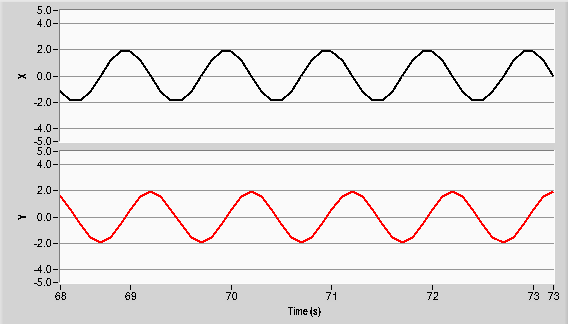
\includegraphics[width=1.2\textwidth]{Chapters/4_Metodología/Imagenes/5.png} \\
    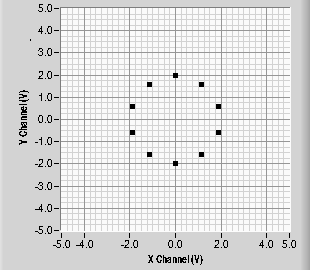
\includegraphics[width=1.2\textwidth]{Chapters/4_Metodología/Imagenes/6.png}
    \end{minipage}} \\
    $f_R$ & 249 \\
    $f_C$ & 60 \\
    $f_{AM}$ & 0\\
    $A_S$ & 2\\
    $A_C$ & 1\\
    $P_{AM}$ & 0\\
    $\eta$ & 0\\
    $\phi$ & 0\\
    $\tau$ & 25m \\
    $V_{MX}$ & 2\\
    $V_{MY}$ & 1\\
    $V_{OutX}$ & 2\\
    $V_{OutY}$ & 2\\
    Entrada sinusoidal & desactivada\\
    Filtro de paso bajo & activado \\
    \hline
\end{tabular}
}
\caption{Variables utilizadas en el simulador con sus respectivas salidas.}
\end{table}


\begin{table}[H]
\centering
\resizebox{0.55\columnwidth}{!}{ % Ajusta el tamaño al 90% del ancho de la columna
\begin{tabular}{c|c|c} % Definir columnas
    \hline
    \textbf{Variable} & \textbf{Valor} & \textbf{Resultados} \\
    \hline
    $f_s$   & 260 & \multirow{6}{*}{%
    \begin{minipage}{.25\textwidth}
    \centering
    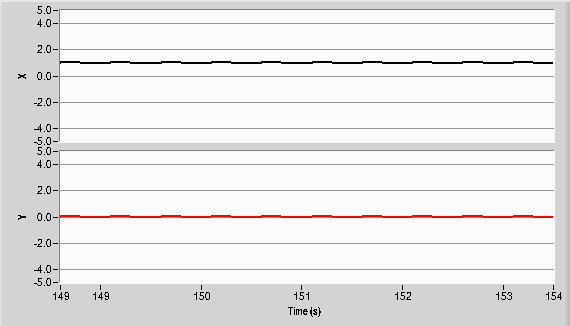
\includegraphics[width=1.2\textwidth]{Chapters/4_Metodología/Imagenes/7.png} \\
    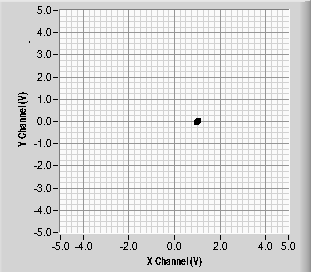
\includegraphics[width=1.2\textwidth]{Chapters/4_Metodología/Imagenes/8.png}
    \end{minipage}} \\
    $f_R$ & 260 \\
    $f_C$ & 2\\
    $f_{AM}$ & 0\\
    $A_S$ & 1\\
    $A_C$ & 3\\
    $P_{AM}$ & 0\\
    $\eta$ & 0\\
    $\phi$ & 0\\
    $\tau$ & 50m \\
    $V_{MX}$ & 4\\
    $V_{MY}$ & 1\\
    $V_{OutX}$ & 1\\
    $V_{OutY}$ & 0\\
    Entrada sinusoidal & activado\\
    Filtro de paso bajo & activado \\
    \hline
\end{tabular}
}
\caption{Variables utilizadas en el simulador con sus respectivas salidas.}
\end{table}

\begin{table}[H]
\centering
\resizebox{0.55\columnwidth}{!}{ % Ajusta el tamaño al 90% del ancho de la columna
\begin{tabular}{c|c|c} % Definir columnas
    \hline
    \textbf{Variable} & \textbf{Valor} & \textbf{Resultados} \\
    \hline
    $f_s$   & 250 & \multirow{6}{*}{%
    \begin{minipage}{.25\textwidth}
    \centering
    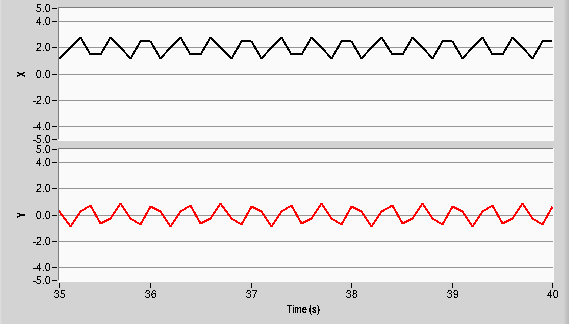
\includegraphics[width=1.2\textwidth]{Chapters/4_Metodología/Imagenes/9.png} \\
    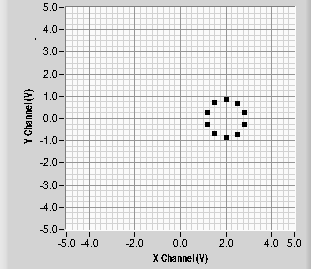
\includegraphics[width=1.2\textwidth]{Chapters/4_Metodología/Imagenes/10.png}
    \end{minipage}} \\
    $f_R$ & 250 \\
    $f_C$ & 253\\
    $f_{AM}$ & 0\\
    $A_S$ & 2\\
    $A_C$ & 1\\
    $P_{AM}$ & 0\\
    $\eta$ & 0\\
    $\phi$ & 0\\
    $\tau$ & 20m \\
    $V_{MX}$ & 3\\
    $V_{MY}$ & 1\\
    $V_{OutX}$ & 3\\
    $V_{OutY}$ & 1\\
    Entrada sinusoidal & activado\\
    Filtro de paso bajo & activado \\
    \hline
\end{tabular}
}
\caption{Variables utilizadas en el simulador con sus respectivas salidas.}
\end{table}


\begin{table}[H]
\centering
\resizebox{0.55\columnwidth}{!}{ % Ajusta el tamaño al 90% del ancho de la columna
\begin{tabular}{c|c|c} % Definir columnas
    \hline
    \textbf{Variable} & \textbf{Valor} & \textbf{Resultados} \\
    \hline
    $f_s$   & 120 & \multirow{6}{*}{%
    \begin{minipage}{.25\textwidth}
    \centering
    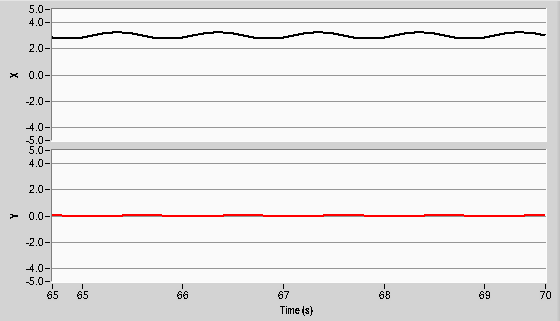
\includegraphics[width=1.2\textwidth]{Chapters/4_Metodología/Imagenes/11.png} \\
    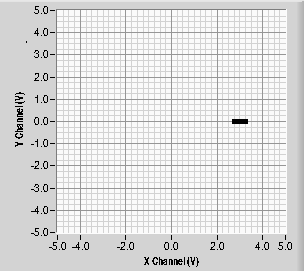
\includegraphics[width=1.2\textwidth]{Chapters/4_Metodología/Imagenes/12.png}
    \end{minipage}} \\
    $f_R$ & 120 \\
    $f_C$ & 253\\
    $f_{AM}$ & 0\\
    $A_S$ & 3\\
    $A_C$ & 1\\
    $P_{AM}$ & 50\\
    $\eta$ & 0\\
    $\phi$ & 0\\
    $\tau$ & 15 \\
    $V_{MX}$ & (4,-4)\\
    $V_{MY}$ & (1,-1)\\
    $V_{OutX}$ & (2.5,3.5)\\
    $V_{OutY}$ & 0\\
    Entrada sinusoidal & desactivado\\
    Filtro de paso bajo & activado \\
    \hline
\end{tabular}
}
\caption{Variables utilizadas en el simulador con sus respectivas salidas.}
\end{table}


Con esto podremos completar los parámetros necesarios para producir las siguientes señales:


\begin{table}[H]
\centering
\resizebox{0.55\columnwidth}{!}{ % Ajusta el tamaño al 90% del ancho de la columna
\begin{tabular}{c|c|c} % Definir columnas
    \hline
    \textbf{Variable} & \textbf{Valor} & \textbf{Resultados} \\
    \hline
    $f_s$   &  & \multirow{6}{*}{%
    \begin{minipage}{.25\textwidth}
    \centering
    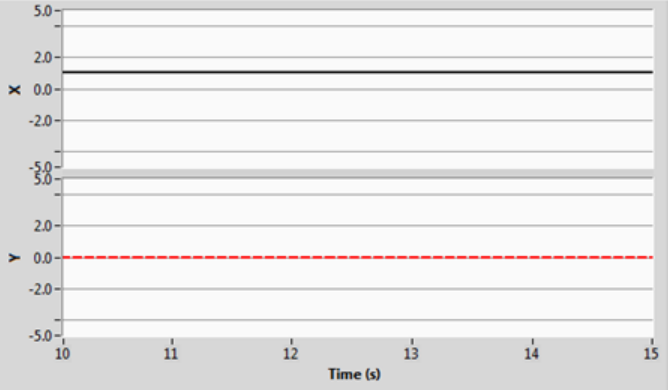
\includegraphics[width=1.2\textwidth]{Chapters/4_Metodología/Imagenes/13.png} \\
    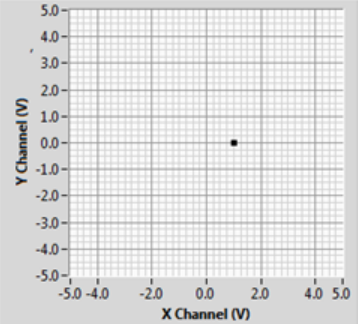
\includegraphics[width=1.2\textwidth]{Chapters/4_Metodología/Imagenes/14.png}
    \end{minipage}} \\
    $f_R$ & 20 \\
    $f_C$ & \\
    $f_{AM}$ & 0\\
    $A_S$ & \\
    $A_C$ & \\
    $P_{AM}$ & 0\\
    $\eta$ & 0\\
    $\phi$ & 0\\
    $\tau$ & 500m \\
    $V_{MX}$ & \\
    $V_{MY}$ & \\
    $V_{OutX}$ & 1\\
    $V_{OutY}$ & 0\\
    Entrada sinusoidal & opcional\\
    Filtro de paso bajo & activado \\
    \hline
\end{tabular}
}
\caption{Primera configuración a resolver utilizando el Simulador LIA.}
\end{table}


\begin{table}[H]
\centering
\resizebox{0.55\columnwidth}{!}{ % Ajusta el tamaño al 90% del ancho de la columna
\begin{tabular}{c|c|c} % Definir columnas
    \hline
    \textbf{Variable} & \textbf{Valor} & \textbf{Resultados} \\
    \hline
    $f_s$   &  & \multirow{6}{*}{%
    \begin{minipage}{.25\textwidth}
    \centering
    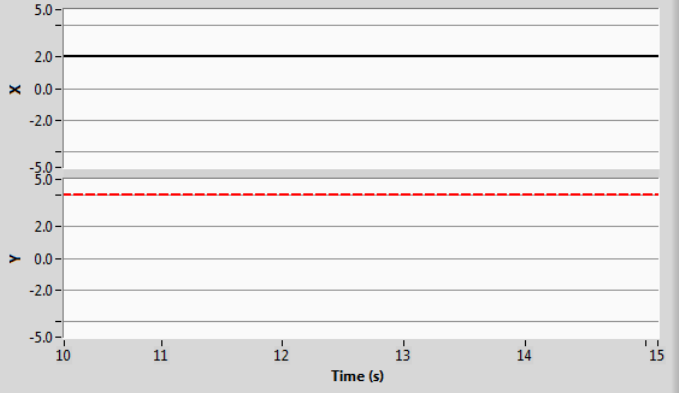
\includegraphics[width=1.2\textwidth]{Chapters/4_Metodología/Imagenes/15.png} \\
    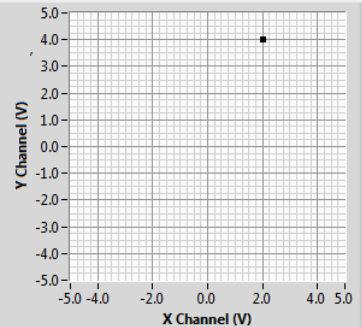
\includegraphics[width=1.2\textwidth]{Chapters/4_Metodología/Imagenes/16.png}
    \end{minipage}} \\
    $f_R$ & 35 \\
    $f_C$ & \\
    $f_{AM}$ & 0\\
    $A_S$ & \\
    $A_C$ & \\
    $P_{AM}$ & 0\\
    $\eta$ & 0\\
    $\phi$ & 0\\
    $\tau$ & 3 \\
    $V_{MX}$ & \\
    $V_{MY}$ & \\
    $V_{OutX}$ & 2\\
    $V_{OutY}$ & 4\\
    Entrada sinusoidal & opcional\\
    Filtro de paso bajo & activado \\
    \hline
\end{tabular}
}
\caption{Segunda configuración a resolver utilizando el Simulador LIA.}
\end{table}


\begin{table}[H]
\centering
\resizebox{0.55\columnwidth}{!}{ % Ajusta el tamaño al 90% del ancho de la columna
\begin{tabular}{c|c|c} % Definir columnas
    \hline
    \textbf{Variable} & \textbf{Valor} & \textbf{Resultados} \\
    \hline
    $f_s$   &  & \multirow{6}{*}{%
    \begin{minipage}{.25\textwidth}
    \centering
    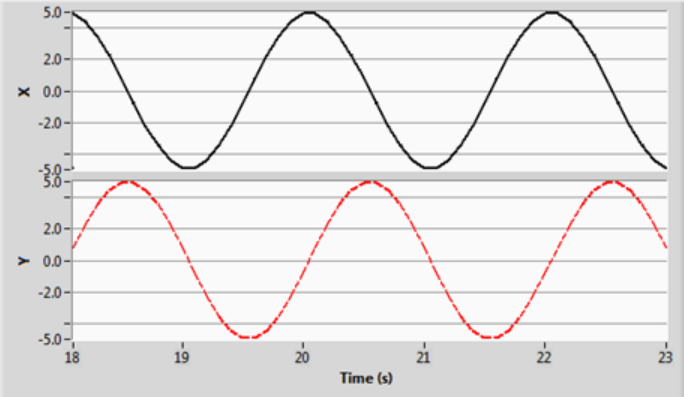
\includegraphics[width=1.2\textwidth]{Chapters/4_Metodología/Imagenes/17.png} \\
    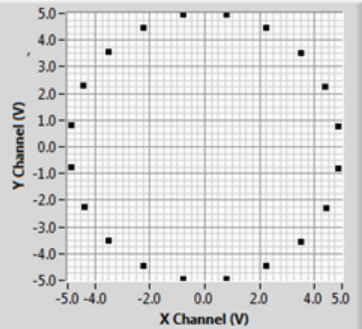
\includegraphics[width=1.2\textwidth]{Chapters/4_Metodología/Imagenes/18.png}
    \end{minipage}} \\
    $f_R$ & 50 \\
    $f_C$ & \\
    $f_{AM}$ & 0\\
    $A_S$ & \\
    $A_C$ & \\
    $P_{AM}$ & 0\\
    $\eta$ & 0\\
    $\phi$ & 0\\
    $\tau$ & 500m \\
    $V_{MX}$ & \\
    $V_{MY}$ & \\
    $V_{OutX}$ & (5,-5)\\
    $V_{OutY}$ & (5,-5)\\
    Entrada sinusoidal & opcional\\
    Filtro de paso bajo & activado \\
    \hline
\end{tabular}
}
\caption{Tercera configuración a resolver utilizando el Simulador LIA.}
\end{table}


\begin{table}[H]
\centering
\resizebox{0.55\columnwidth}{!}{ % Ajusta el tamaño al 90% del ancho de la columna
\begin{tabular}{c|c|c} % Definir columnas
    \hline
    \textbf{Variable} & \textbf{Valor} & \textbf{Resultados} \\
    \hline
    $f_s$   &  & \multirow{6}{*}{%
    \begin{minipage}{.25\textwidth}
    \centering
    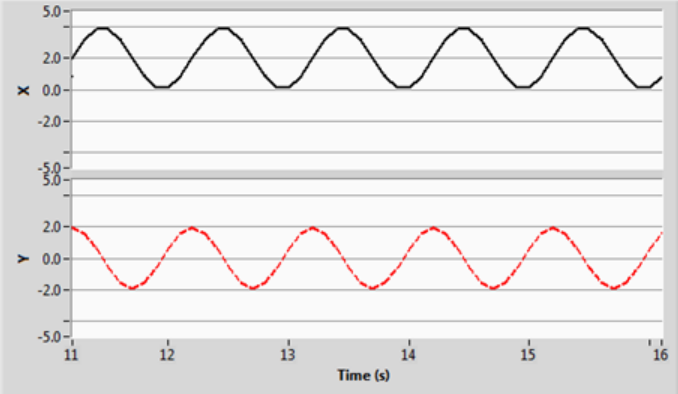
\includegraphics[width=1.2\textwidth]{Chapters/4_Metodología/Imagenes/19.png} \\
    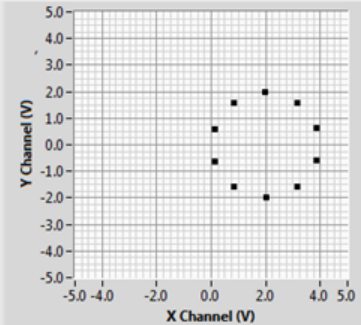
\includegraphics[width=1.2\textwidth]{Chapters/4_Metodología/Imagenes/20.png}
    \end{minipage}} \\
    $f_R$ & 0.50 \\
    $f_C$ & \\
    $f_{AM}$ & 0\\
    $A_S$ & \\
    $A_C$ & \\
    $P_{AM}$ & 0\\
    $\eta$ & 0\\
    $\phi$ & 0\\
    $\tau$ & 20m \\
    $V_{MX}$ & \\
    $V_{MY}$ & \\
    $V_{OutX}$ & (0,4)\\
    $V_{OutY}$ & (2,-2)\\
    Entrada sinusoidal & opcional\\
    Filtro de paso bajo & activado \\
    \hline
\end{tabular}
}
\caption{Cuarta configuración a resolver utilizando el Simulador LIA.}
\end{table}


Continuando con las etapas de medición con el simulador, se muestran las simulaciones ejecutas en esta etapa:


\begin{table}[H]
\centering
\resizebox{0.55\columnwidth}{!}{ % Ajusta el tamaño al 90% del ancho de la columna
\begin{tabular}{c|c|c} % Definir columnas
    \hline
    \textbf{Variable} & \textbf{Valor} & \textbf{Resultados} \\
    \hline
    $f_s$   & 10 & \multirow{6}{*}{%
    \begin{minipage}{.25\textwidth}
    \centering
    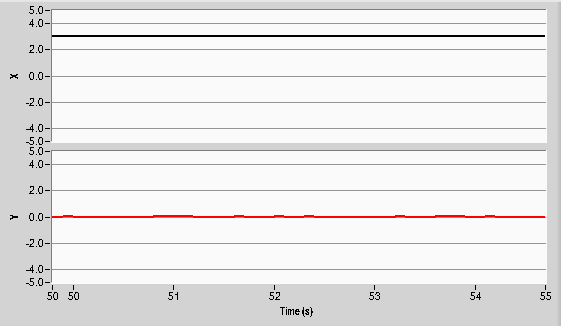
\includegraphics[width=1.3\textwidth]{Chapters/4_Metodología/Imagenes/1s.png} \\
    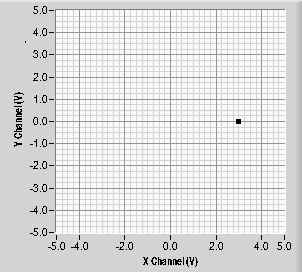
\includegraphics[width=1.3\textwidth]{Chapters/4_Metodología/Imagenes/2s.png}
    \end{minipage}} \\
    $f_R$ & 10 \\
    $f_C$ & 60\\
    $f_{AM}$ & 0\\
    $A_S$ & 3\\
    $A_C$ & 1\\
    $P_{AM}$ & 0\\
    $\eta$ & 0\\
    $\phi$ & 0\\
    $\tau$ & 2 \\
    $V_{MX}$ & (3,-3)\\
    $V_{MY}$ & (1,-1)\\
    $V_{OutX}$ & 3\\
    $V_{OutY}$ & 0\\
    Entrada sinusoidal & desactivado\\
    Filtro de paso bajo & activado \\
    Seguimiento automático & desactivado\\
    \hline
\end{tabular}
}
\caption{Simulación 1: Demostrando uno de los usos más comunes del amplificador lock-in. Medir la amplitud de una frecuencia específica en la señal de entrada configurando $f_S=f_R$.
}
\end{table}





%%%%%%%%%%%%%%%%%%%%%%%%%%%%%%%%%%%%%%%%%%%%%%%%%%%%%%%%%%%%%%%%
\newpage
 